\section{Discussion}
\label{sect:discussion}

\begin{figure}
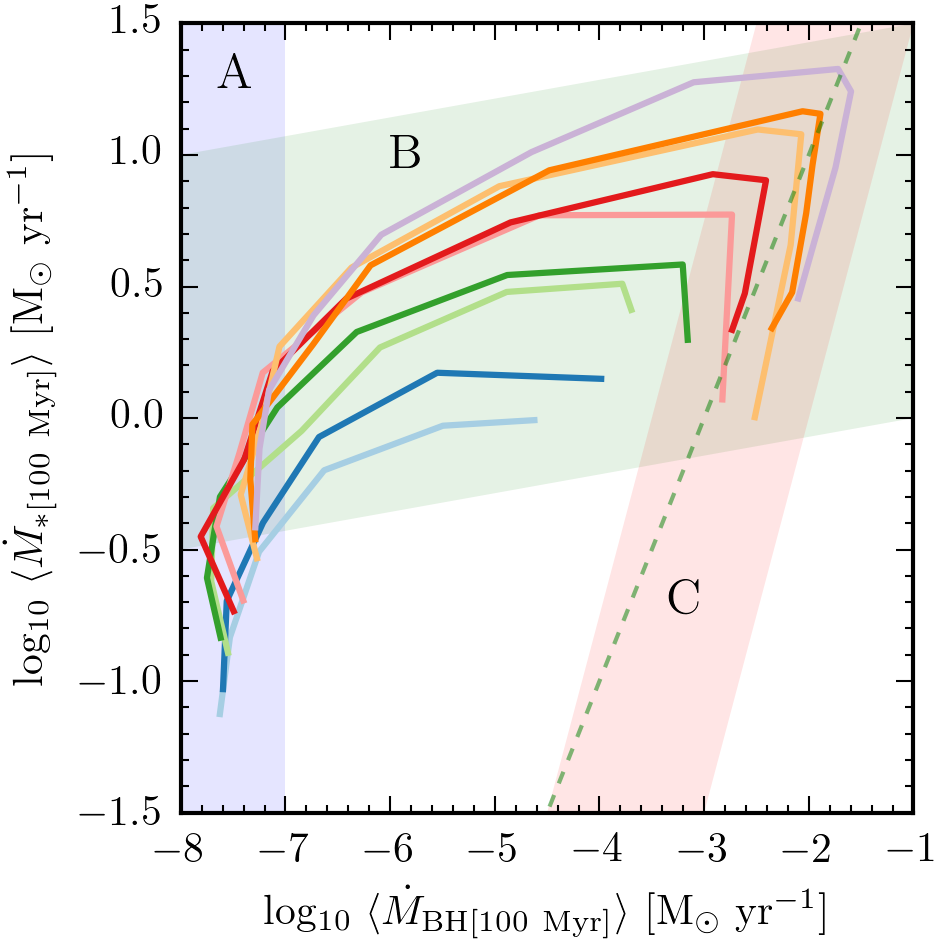
\includegraphics[width=\columnwidth]{plots/AvSFRvsBHAR}

\caption{Each line shown here equates the median trends from the top two panels
of \cref{fig:avHistory_vs_hm} to give the 100~Myr average SFR as a function of
the 100~Myr average BHAR (in equal spacings of halo mass). Region \emph{A}
(shaded blue) corresponds to galaxies hosted by haloes with \M{200}
$\lesssim$\M{crit}. Galaxies in this regime increase their SFR with increasing
halo mass, while BHARs remain negligible on average. As haloes reach
$\sim$\M{crit} in region \emph{B} (shaded green), SFRs continue to rise,
however the BH growth increases by many orders of magnitude over this narrow
halo mass range. For haloes in excess of $\gtrsim$ \M{crit} shown in region
\emph{C} (shaded red), we see a reduction for both SFR and BHAR on average,
yielding a approximately constant scaling between the two growth rates (compare
to dashed green line which shows the linear relation \BHAR/\SFR = $10^{-3}$).}

\label{fig:sfr_vs_bhar_av} \end{figure}

Throughout this investigation we have consistently found no evidence supporting
a simple underlying relationship between the rate of a galaxy's star formation
and the accretion rate of its central BH. Instead, a mutual dependence of each
property upon the mass of the host halo yields a more complex connection. It is
interesting to examine, then, how the relation between the SFR and BHAR evolves
for individual objects. In the following discussion, we will provide a physical
interpretation based on the \citet{Bower2017} (hereafter B16) model for BH
growth \citep[for a similar interpretation on the importance of SN feedback to
BH growth see][]{Dubois2015,Habouzit2016}.  However, we stress the simulation
results are themselves independent of any physical interpretation.  

\cref{fig:sfr_vs_bhar_av} equates the median trends of the SFR and BHAR
histories shown in \cref{fig:avHistory_vs_hm}. This specifies the 100~Myr
average SFR as a function of the 100~Myr average BHAR in equal spacings of halo
mass.  Three distinct trends between SFR and BHAR emerge as the halo evolves:
the \emph{stellar feedback regulated} phase (shaded blue), the \emph{non-linear
BH growth} phase (shaded green) and the \emph{AGN feedback regulated} phase
(shaded red).

\begin{itemize}

\item \emph{Region A - The stellar feedback regulated phase}: From the time of
their seeding until they are hosted by haloes of mass \M{200} $\sim
10^{11.5}$\Msol the BH accretion rates are negligible (\BHAR $\leq
10^{-6}$\Msolyr on average).  By contrast, SFRs increase steadily with halo
mass. This behaviour produces the uncorrelated (yet causally connected)
$\sim$vertical trend in region \emph{A}, creating an imbalance of growth within
these systems. As a result, BHs remain close to their seed mass whilst the
halo/galaxy continues to grow around them (see the low-mass region of
\cref{fig:bhm_vs_hm}).

B16 interpret galaxies in this regime as being in a state of regulatory
equilibrium. Energy injected by stars heats the ISM within the stellar vicinity,
ejecting it, and causing it to rise buoyantly in the halo. This in turn creates
an outflow of material balancing the freshly sourced fuel from the cosmic web,
and as such prevents large gas densities from building up within the inner
regions of these low-mass galaxies.  Such low densities, coupled with the
relatively low mass BHs living within these galaxies (BHAR $\propto
M_{\mathrm{BH}}^{2}$), ensures that BHs fail to grow substantially. 

\item \emph{Region B - The non-linear BH growth phase}: Both galaxies and BHs
grow through the halo mass range \M{200} $\sim 10^{11.5} - 10^{12.0}$\Msol.
However, whereas the SFRs continue to increase steadily with increasing halo
mass, BHs rapidly transition to a non-linear phase of growth. This creates a
highly non-linear \textit{indirect} correlation between SFR and BHAR, connected
through the host halo mass.  

The physical interpretation posited by B16 is that haloes that grow to the
transition mass, \M{crit}, have become sufficiently massive to stall the
regulatory outflow. Due to (what is now) the halos' hot coronae, heated gas
ejected by stellar feedback loses the capability to rise buoyantly and
therefore returns to the galaxy centre.  Densities in the central regions of
the galaxy are no longer kept low and a \squotes{switch} to non-linear BH
growth is triggered.  

\item \emph{Region C - The AGN feedback regulated phase}: For haloes with
masses above \M{200} $\sim 10^{12}$\Msol SFRs and BHARs both decline on
average, correlated with an approximately linear trend (compare to green dashed
line, see also bottom panel of \cref{fig:avHistory_vs_hm}). 

B16 argue that BHs in these haloes have become sufficiently massive (through
their rapid non-linear growth) to efficiently regulate the gas inflow onto the
galaxy themselves via AGN feedback.  This again creates an equilibrium state,
for which a fluctuating low level of (specific) BH accretion is maintained,
keeping the outer halo hot and evaporating much of the new cold material trying
to enter the system from the intergalactic medium.

\end{itemize}

Galaxies and their central BHs within the \eagle simulation transition through
multiple stages of growth as their host dark matter halo evolves, creating
three distinct behaviours between SFR and BHAR. This is a stark contrast to a
simple model where SFR and BHAR correlate globally via a linear relation, on
average and for all halo masses. Whilst the underlying trend is only revealed
when each growth rate is time-averaged (given the inherent noise of
instantaneous growth rates), we only find an approximately linear correlation
for the most massive systems (\M{200} $\gtrsim 10^{12.5}$\Msol).

In this paper we have emphasised the role of the halo and how its interaction
with both SFR and BHAR shapes the growth rate relationship.  However,
additional factors may also contribute to the form this relationship takes. For
example, \citet{Volonteri2015b} find using a suite of isolated merger
simulations at fixed halo mass, that alternate behaviours between SFR and BHAR
before, during and after the merger proper collectively contribute to form a
complex two-dimensional plane.  Additionally, \citet{Pontzen2017} reveal the
particular importance differing merger histories can have on significantly
altering the growth rate history of both that of the galaxy and the central BH.
However, the global influence of mergers upon galaxy and BH growth rates in a
full cosmological context remains open for debate, and will be the subject of a
future paper. 

